\section{Methodology} \label{tex:methodology}
Overall the methods examined in this thesis can be divided into two parts; namely those trying to decompose the input into a NN, and those decomposing the weights of a pre-trained NN with subsequent fine-tuning. In the following the methods used within each of these parts will be discussed in detail. All decomposition estimation will be executed using the Python library \textit{TensorLy}\cite{tensorly}, which provides an application programming interface (API) for tensor methods using different back-ends\footnote{The back-end is the Python library that is responsible for low-level calculation and specification of the tensors. Typically \textit{NumPy}\cite{numpy} or \textit{PyTorch}\cite{pytorch}} for calculations. The algorithms for estimating the decompositions are given in \autoref{app:DecompEstimation}. 

\subsection{Decomposing the Input}
In reality, tampering with data that is going to be learned is data preprocessing, hence decomposing the input is just a form of this. Data preprocessing is a vital part of almost all ML, because structured data of high quality is simply much easier to learn and to work with. Put in another way: "Garbage in, garbage out". In addition knowledge of the structure and the variance of the data often ease the algorithm development process. The decomposition algorithms seems appropriate for this task due to their ability to exploit the structure of the data.

The Tucker decomposition is believed to be suitable for data compression tasks \cite{Mørup2011}, which is why it seems natural to apply this method to the data before feeding it in to and training the NN. The purpose is to let the decomposition do some of the learning beforehand by exploiting the variance in the data. The Tucker-decomposition is flexible since it allows for decomposition of only a subset of the dimensions\footnote{This is also called a \textit{partial} Tucker decomposition}, and because it allows for specification of ranks for each dimension individually. Since the ranks correspond to the degree of flexibility, it is easy to choose how flexible the decomposition should be along each dimension. The rank would increase with the level of desired detail. This means that if the goal of the algorithm is to differentiate a small set of features, the rank would also be kept small along the relevant dimension.

Since the observations in each the given data sets can be stacked to form a 4 (MNIST) or 5 (THETIS) dimensional tensor, it is fairly straight forward to apply the Tucker decomposition. For $N$ MNIST observations, the stacked tensor $\tensor{X}$ of size $(N \times 1 \times 28 \times 28)$ will be reshaped to $(N\times 28 \times 28)$ due to the single input channel. The decomposition of the now 3rd order tensor becomes:
\begin{equation}
    \tensor{X}^{N\times 28 \times 28} \ \approx \  \tensor{G}^{L\times J \times K} \times_1 \bs{A}^{N\times L} \times_2 \bs{B}^{28 \times J} \times_3 \bs{C}^{28 \times K}
\end{equation}
Where $L, J$ and $K$ corresponds to the ranks in each of the dimensions. Here $\tensor{G}$ is the core of the decomposition, $\bs{A}$ corresponds to the loading matrix along the between-sample dimension, while $\bs{B}$ and $\bs{C}$ correspond to the loading matrices in each of the spatial dimensions. Since the goal is to learn the differences between the different digits in the data set, we will only decompose the between-sample dimension. The so-called Tucker-1 decomposition of the first dimension is given by:
\begin{equation}
    \tensor{X}^{N\times 28 \times 28} \ \approx \  \tensor{G}^{L\times 28 \times 28} \times_1 \bs{A}^{N\times L} \times_2 \bs{I}^{28 \times 28} \times_3 \bs{I}^{28 \times 28}
\end{equation}
Now the loading matrix $\bs{A}$ holds information about what differentiates the different samples using only $L$ features. These features will be used as the input into a simple ANN, potentially lowering the number of input nodes dramatically if $L$ is kept small. The algorithm is summarized in XX. 

\subsubsection{Estimating the decomposition for the testing data}
Since the testing data cannot be decomposed with the training data, the loading matrix for the testing data will be estimated assuming the same core as for the training data. This way the decomposition is also a part of the training. Based on \eqref{eq:tuckerMNISTinput} the loading matrix for the test set can be estimated by multiplying with the pseudo-inverse of the matricized core:
\begin{equation}
    \bs{A}_{test} \approx \bs{X}_{test_{(1)}} \bs{G}_{(1)}^{\ \dagger}
\end{equation}
The two matrices $\bs{A}$ and $\bs{A}_{test}$ will be given as the input to a very simply ANN as the training data and the validation/testing data respectively.


%%%%%%%%%%%%%%%%%%%%%%%%%%%%%%%%%%%%%%%%%%%%%%%%%%%%%%%%%%%%%%%%%%%%%%%%%%%%%%%%%%%%    Decomposing Pre-Trained Network    %%%%%%%%%%%%%%%%%%%%%%%%%%%%%%%%%%%%%%%
%%%%%%%%%%%%%%%%%%%%%%%%%%%%%%%%%%%%%%%%%%%%%%%%%%%%%%%%%%%%%%%%%%%%%%%%%%%%%%%%%

\subsection{Decomposing a Pre-Trained Network}
Using this approach is relatively easy to justify which is properly the reason why all the methods discussed in \autoref{tex:previous_work} use this approach. Pre-training a network makes it easier to ensure a network that works well, also because the training is often performed on powerful computers which allows for more complex networks. After the training is concluded the network is only decomposed to optimise the evaluation time in order to make it useful on platforms with less computation power. As discussed in \autoref{tex:previous_work} there are multiple approaches for this, but especially the methods using Tucker-decomposition and BTD seamed to be performing well and relatively straight-forward to implement and fine-tune. In this section the algorithms and implementation, used in this thesis, will be discussed. 

\subsubsection{Compressing entire CNN using Tucker decomposition}
This method builds on the work done by Kim et al. in \cite{Kim2016}, which is briefly discussed in \autoref{tex:sub_entire_network}.  Similar to the work done by Kim et al., Tucker-1 or Tucker-2 will be used for specific layers through the network. Due to the dissimilarities of the linear layer and the convolutional layer, each of these decompositions will be implemented individually for each type of layer.

\paragraph{The linear layer}
As explained in XX the linear layer with $N_{in}$ input neurons and $N_{out}$ output neurons in simply a matrix-vector product:
\begin{equation}
    \bs{y}^{N_{out}} = \bs{W}^{N_{out}\times N_{in}}\bs{x}^{N_in} + \bs{b}^{N_{out}}
    \label{eq:linearLayerTransformWOdecomp}
\end{equation}
Where $\bs{x}$ is the input, $\bs{y}$ is the input, $\bs{b}$ is the bias vector, and $\bs{W}$ is the weight matrix. The weight matrix is potentially big resulting in many parameters and high calculation time. The idea of the decomposed linear layer is to decompose the weight tensor into a set of smaller matrices that can be multiplied sequentially resulting in higher efficiency. The Tucker-1 and Tucker-2 decompositions of the weight matrix are given as:
\begin{align}
\texttt{Tucker-1}&: \quad \bs{W} \approx \bs{G} \times_1 \bs{A} \times_2 \bs{I} = \bs{A}\bs{G} \qquad \text{OR} \qquad \bs{W} \approx \bs{G} \times_1 \bs{I} \times_2 \bs{B} = \bs{G}\bs{B}^\top \\
\texttt{Tucker-2}&: \quad \bs{W} \approx \bs{G} \times_1 \bs{A} \times_2 \bs{B} = \bs{A}\bs{G}\bs{B}^\top 
\end{align}
Here $\bs{I}$ is the identity matrix and the core tensor $\bs{G}$ is a matrix due to the weight matrix $\bs{W}$ only having 2 dimensions. The type of Tucker-1 decomposition is chosen based on which dimension is to be decomposed.\footnote{Dense layers often go from many inputs to a fewer outputs why the input dimension might be more desirable to compress} Inserting the decomposition of $\bs{W}$ in the linear transform \eqref{eq:linearLayerTransformWOdecomp} yields:
\begin{align*}
     \bs{y}^{N_{out}} &\approx \bs{A}^{N_{out}\times R_A} \bs{G}^{R_A\times N_{in}} \bs{x}^{N_{in}} + \bs{b}^{N_{out}} \\
    \texttt{Tucker-1}: \qquad \quad \ \ &\text{OR} \\
    \bs{y}^{N_{out}} &\approx \bs{G}^{N_{out}\times R_B} \bs{B}^{\top \  R_B\times N_{in}}\bs{x}^{N_{in}} + \bs{b}^{N_{out}} \\
    &\quad \\
    \texttt{Tucker-2}: \quad \bs{y}^{N_{out}} &\approx \bs{A}^{N_{out}\times R_A} \bs{G}^{R_A\times N_{in}} \bs{B}^{\top  R_B\times N_{in}}\bs{x}^{N_{in}} + \bs{b}^{N_{out}}
\end{align*}
Now looking at the number of multiplications needed to do each of the products from right to left gives the values in \autoref{tab:numberOfMultiplicationsLinearLayer}. For instance using the Tucker-1 compression uses $N_{in}R + RN_{out}=R(N_{out}+N_{in})$ multiplications to do the matrix-product. The table also shows the restrictions on the ranks to have less multiplications than the uncompressed version, hence to be more efficient.
\begin{table}
    \centering
    \captionsetup{width=.9\linewidth}
    \caption{The number of multiplications needed to do the matrix-vector product in the linear layer \eqref{eq:linearLayerTransformWOdecomp} with the weight matrix decomposed using Tucker-1 and Tucker-2. The matrix product is assumed to be calculated from right to left.}
    \begin{tabular}{l|c|c}
        \textbf{Method} & \textbf{\# Multiplications} & \textbf{Faster when:} \\ \hline
        Uncrompressed & $N_{out} N_{in}$ & - \\
        Tucker-1 & $R(N_{in} + N_{out})$ & $R < \frac{N_{out}N_{in}}{N_{out} + N_{in}}$\\
        Tucker-2 & $N_{in}R_B + R_BR_A + R_AN_{out}$ & $(N_{in}+R_A)(N_{out}+R_B) < 2 N_{in}N_{out}$
    \end{tabular}
    \label{tab:numberOfMultiplicationsLinearLayer}
\end{table}

What also makes this decomposition smart is that the sequence of matrix multiplications can be achieved by a sequence of 2 or 3 linear layers, where the loadings from the decomposition can be directly used as weights. This makes it straight-forward to adapt the layer into a decomposed version and to fine-tune. The concept is illustrated in \autoref{fig:diffNNlinearLayer}. The biases from the original layer will be added only to the last layer in the sequence of the decomposed version and they will not be modified in any way.
\begin{figure}
    \centering
    \begin{subfigure}{0.35\linewidth}
        \centering
        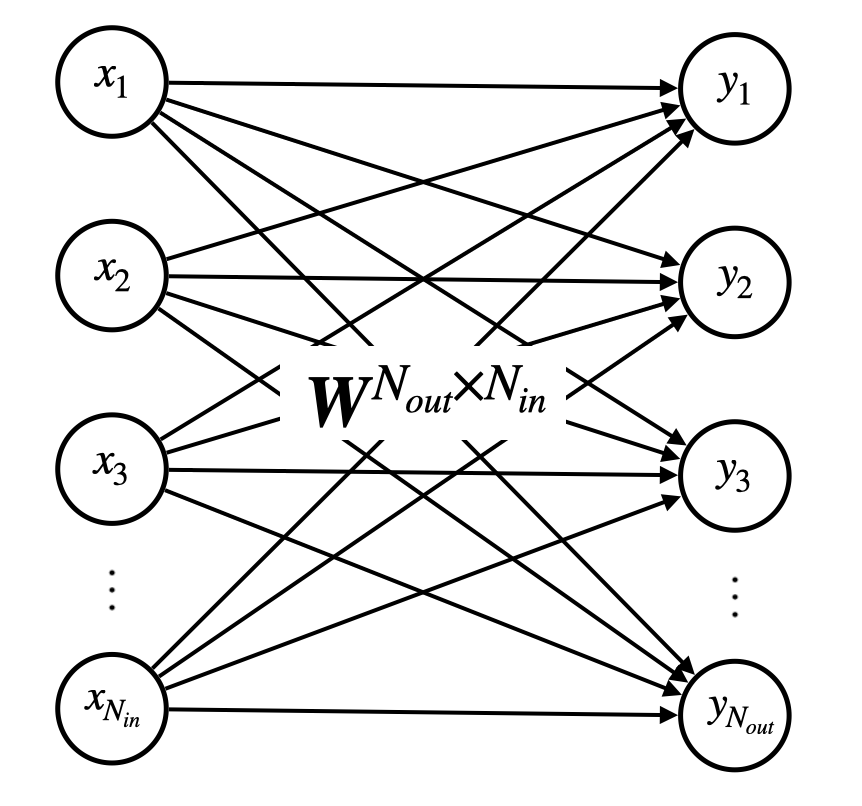
\includegraphics[width=\linewidth]{Pics/05_methodology/NNlinearLayer.png}
        \caption{Original linear layer}
    \end{subfigure}
    \begin{subfigure}{\linewidth}
        \centering
        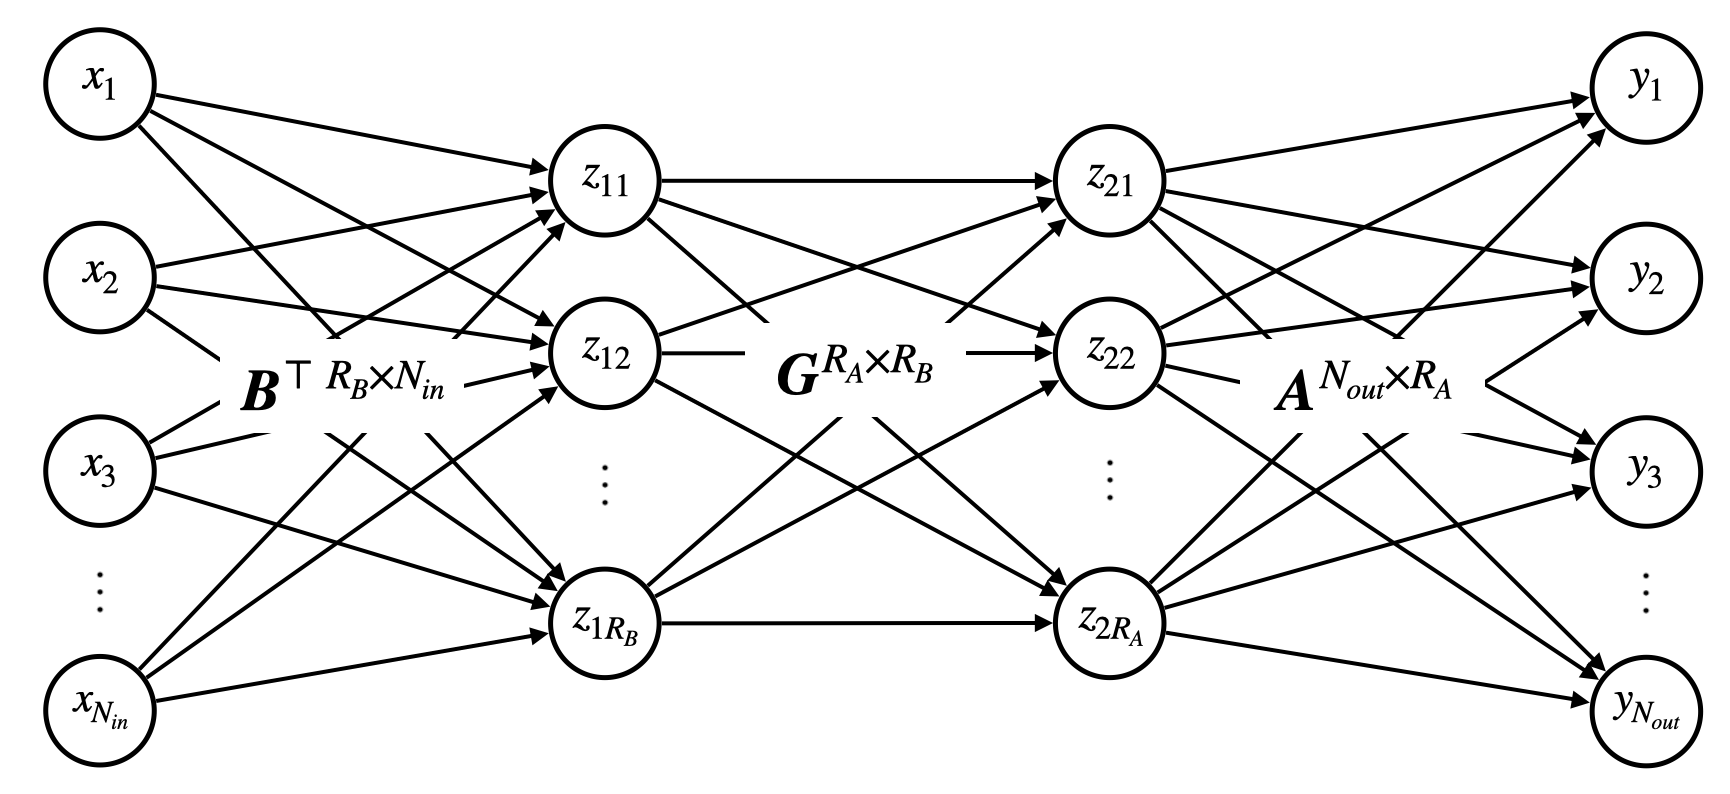
\includegraphics[width=.7\linewidth]{Pics/05_methodology/NNdecompLinearLayer.png}
        \caption{Sequence of linear layers resulting after decomposing $\bs{W}$}
    \end{subfigure}
    \captionsetup{width=.9\linewidth}
    \caption{Illustration of the difference between the original linear layer and the decomposed sequence of linear layers. The matrices $\bs{A}, \bs{B}$ and $\bs{G}$ are the resulting loading matrices and core respectively after decomposing the original weight matrix $\bs{W}$. The biases from the original layer will be added only to the last layer in the decomposed sequence.}
    \label{fig:diffNNlinearLayer}
\end{figure}

\paragraph{The convolutional layer}